% ============================================================
% Chapter 12 — Low-Volume Production Economics
% Folder: chapters/12-economics
% Course: Project Planning & Prototyping (247-519-VA, Vanier College)
% ============================================================

\chapter{Low-Volume Production Economics}
\label{ch:economics}

\paragraph{Where this fits.}
Chapter~11 delivered a validated prototype and a costed Bill of Materials for the IoT robotic sorting subsystem; this chapter sits at Gate~3 of the Stage-Gate model and fills the gap between that one-off prototype cost and the production economics that underpin the go/kill decision.
A team that passes Gate~3 has demonstrated a working prototype and a credible
BOM; the gate committee now asks a harder question: \emph{can this product be
made and sold profitably?}
The cost projection produced in this chapter is the economic half of that
answer.
Gate~3 reviewers will scrutinise your unit-cost curve and break-even analysis
as carefully as they scrutinise your test results.


\paragraph{Learning Objectives.}
\begin{enumerate}
  \item Compute and plot the unit-cost curve $C_{\text{unit}}(N)$ from a
        prototype BOM and an estimated fixed cost.
  \item Find the break-even volume $N^{*}$ between two competing production
        processes.
  \item Connect design decisions made at Stage~3 to downstream manufacturing
        cost, using the DFM/DFA framework introduced in Chapter~7.
\end{enumerate}

% ─────────────────────────────────────────────────────────────────────────────
\section{Why Low-Volume Bridge Production Exists}
\label{sec:ch12-bridge}
% ─────────────────────────────────────────────────────────────────────────────

Between a validated prototype and a full production run lies a zone that
engineers call \textbf{bridge production}\index{bridge production} or
\textbf{low-volume production}\index{low-volume production}.
Volumes in this zone are typically 10 to 500 units --- too many to hand-build
one at a time, too few to justify the tooling cost of high-volume manufacturing.

Bridge production serves three purposes.
First, it generates the first real product units for pilot customers, whose
feedback feeds directly back into the design before a large capital commitment
is made.
Second, it exposes assembly and yield problems that never appear in a
single-unit prototype, where defects are caught and reworked by the same
engineer who built the board.
Third, it provides the actual cost data that replaces the estimates in the
Gate~3 projection.

\paragraph{In Practice.}
Many hardware startups and college capstone projects skip bridge production
entirely: they build one prototype, quote a retail price, and claim the product
is viable.
The prototype BOM is then mistaken for the unit cost.
The result is a Gate~3 slide showing a \$226 unit cost for a product priced at
\$300 --- a margin of 25\,\% that evaporates as soon as a contract manufacturer
quotes assembly labour, packaging, and regulatory compliance.

% ─────────────────────────────────────────────────────────────────────────────
\section{Fixed vs.\ Variable Cost}
\label{sec:ch12-fixed-variable}
% ─────────────────────────────────────────────────────────────────────────────

Every cost in a production run belongs to one of two categories.

\textbf{Variable cost}\index{variable cost} ($c_{\text{var}}$) is the cost that
changes in proportion to the number of units produced.
Components, raw materials, and direct assembly labour are variable: build one
more unit and you spend $c_{\text{var}}$ more.
For the sorting subsystem, Chapter~11 established $c_{\text{var}} = \$480$~CAD,
which reflects component cost plus estimated assembly labour at production
volume.

\textbf{Fixed cost}\index{fixed cost} ($C_{\text{fixed}}$) is the cost paid
once, regardless of how many units are produced.
Tooling (injection-mould tools, PCB test fixtures, jigs), non-recurring
engineering (NRE) charges from a contract manufacturer, certification fees, and
software licences are fixed: doubling the run does not double these costs.
For the sorting subsystem, $C_{\text{fixed}} = \$8{,}000$~CAD, which covers the
PCB test fixture (\$2,400), the injection-mould tool for the housing
(\$4,800), and NRE setup charges (\$800).

\noindent\textbf{Common Pitfalls.}
Three errors appear consistently in student Gate~3 submissions.

\begin{enumerate}
  \item[(a)] \textbf{Treating prototype unit cost as production unit cost.}
        The prototype BOM (\$226) includes retail component prices and one-off
        shipping.
        At volume, component prices drop and shipping is amortised; variable
        cost and prototype cost are different quantities.
  \item[(b)] \textbf{Forgetting that $c_{\text{var}}$ excludes fixed costs.}
        The formula for $C_{\text{unit}}$ (see Section~\ref{sec:ch12-unit-cost})
        adds fixed costs explicitly; if you fold tooling into your variable cost
        estimate you will double-count it.
  \item[(c)] \textbf{Omitting hidden fixed costs.}
        Certification (CE, FCC, CSA) and first-article inspection are fixed costs
        that do not scale.
        A product sold in Canada and shipped to the US carries two regulatory
        budgets.
\end{enumerate}

% ─────────────────────────────────────────────────────────────────────────────
\section{The Unit-Cost Curve}
\label{sec:ch12-unit-cost}
% ─────────────────────────────────────────────────────────────────────────────

When $C_{\text{fixed}}$ is spread over $N$ units and $c_{\text{var}}$ is paid
per unit, the total cost of a run of $N$ units is

\[
  C_{\text{total}}(N) = C_{\text{fixed}} + N \cdot c_{\text{var}}.
\]

Dividing by $N$ gives the \textbf{unit cost}\index{unit cost}:

\begin{equation}
  C_{\text{unit}}(N) = \frac{C_{\text{fixed}}}{N} + c_{\text{var}}.
  \label{eq:ch12-unit-cost}
\end{equation}

Equation~\ref{eq:ch12-unit-cost} is a rectangular hyperbola in $N$.
As $N \to \infty$, $C_{\text{unit}}$ asymptotes to $c_{\text{var}}$ from above:
no matter how large the run, you cannot drive unit cost below the variable cost
per unit.
At $N = 1$, unit cost equals $C_{\text{fixed}} + c_{\text{var}}$: the entire
tooling and setup burden falls on a single unit.

Figure~\ref{fig:ch12-unit-cost-curve} illustrates this relationship for the
sorting subsystem.

\begin{figure}[htbp]
  \centering
  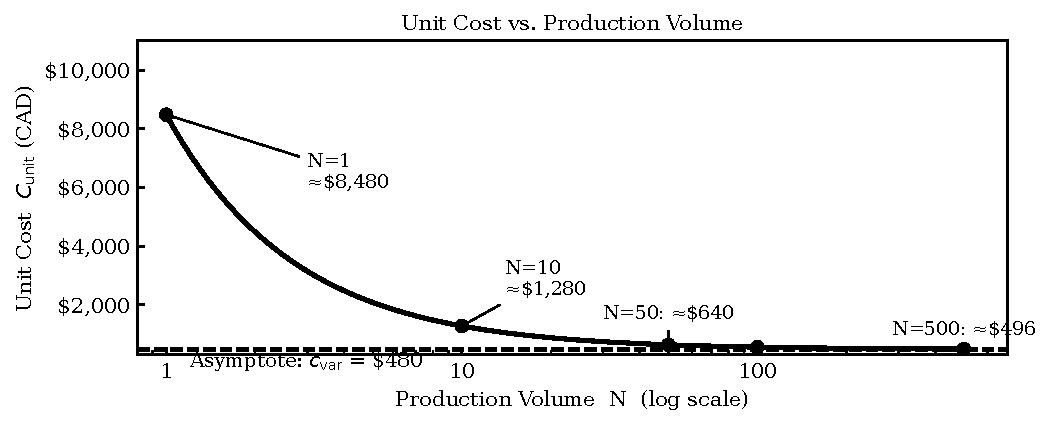
\includegraphics[width=0.82\textwidth]{images/fig_01_unit_cost_curve}
  \caption{$C_{\text{unit}}(N)$ for the IoT sorting subsystem
           ($C_{\text{fixed}} = \$8{,}000$~CAD, $c_{\text{var}} = \$480$~CAD).
           The curve is a rectangular hyperbola that asymptotes to \$480 as
           volume grows.
           The dashed horizontal line marks the \$480 asymptote;
           the dotted vertical line marks $N = 80$, where the fixed-cost
           contribution falls to \$100 per unit.}
  \label{fig:ch12-unit-cost-curve}
\end{figure}

\subsection{Worked Example A: Computing the Unit-Cost Table}
\label{sec:ch12-worked-a}

Given $C_{\text{fixed}} = \$8{,}000$~CAD and $c_{\text{var}} = \$480$~CAD,
apply Equation~\ref{eq:ch12-unit-cost} at five production volumes.

\medskip
\noindent\textbf{$N = 1$:}
\[
  C_{\text{unit}}(1) = \frac{8{,}000}{1} + 480 = 8{,}000 + 480
  = \$8{,}480\text{ CAD.}
\]

\noindent\textbf{$N = 10$:}
\[
  C_{\text{unit}}(10) = \frac{8{,}000}{10} + 480 = 800 + 480
  = \$1{,}280\text{ CAD.}
\]

\noindent\textbf{$N = 50$:}
\[
  C_{\text{unit}}(50) = \frac{8{,}000}{50} + 480 = 160 + 480
  = \$640\text{ CAD.}
\]

\noindent\textbf{$N = 100$:}
\[
  C_{\text{unit}}(100) = \frac{8{,}000}{100} + 480 = 80 + 480
  = \$560\text{ CAD.}
\]

\noindent\textbf{$N = 500$:}
\[
  C_{\text{unit}}(500) = \frac{8{,}000}{500} + 480 = 16 + 480
  = \$496\text{ CAD.}
\]

\medskip
These five values are collected in Table~\ref{tab:ch12-unit-cost}.

\begin{table}[htbp]
  \centering
  \caption{Unit cost at selected production volumes
           ($C_{\text{fixed}} = \$8{,}000$~CAD, $c_{\text{var}} = \$480$~CAD).}
  \label{tab:ch12-unit-cost}
  \begin{tabular}{rrrrr}
    \hline
    $N$ & $C_{\text{fixed}}/N$ & $c_{\text{var}}$ & $C_{\text{unit}}$ & Gross margin at $p=\$1{,}200$ \\
    \hline
      1 & \$8{,}000 & \$480 & \$8{,}480 & $-$606\,\% \\
     10 & \$800     & \$480 & \$1{,}280 & $-$6.7\,\% \\
     50 & \$160     & \$480 & \$640     & 46.7\,\%   \\
    100 & \$80      & \$480 & \$560     & 53.3\,\%   \\
    500 & \$16      & \$480 & \$496     & 58.7\,\%   \\
    \hline
  \end{tabular}
\end{table}

\noindent Notice the rapid improvement between $N = 1$ and $N = 50$: the unit
cost falls by \$7,840 in that interval, compared with only \$144 in the
interval from $N = 50$ to $N = 500$.
The curve is steep at low volume and flat at high volume --- this is the
economic signature of the hyperbola.

\medskip
\noindent\textbf{At what $N$ does the fixed-cost contribution fall below
\$100?}

Set the fixed-cost contribution equal to \$100 and solve for $N$:
\[
  \frac{C_{\text{fixed}}}{N} = 100
  \implies N = \frac{C_{\text{fixed}}}{100} = \frac{8{,}000}{100} = 80
  \text{ units.}
\]

At $N = 80$ the fixed cost adds exactly \$100 per unit; below 80 units each
unit carries more than \$100 of tooling burden.
This threshold is marked in Figure~\ref{fig:ch12-unit-cost-curve}.

% ─────────────────────────────────────────────────────────────────────────────
\section{Process Break-Even}
\label{sec:ch12-breakeven}
% ─────────────────────────────────────────────────────────────────────────────

Different manufacturing processes carry different cost structures.
A process with low fixed cost but high variable cost (such as 3D printing)
is cheapest at low volume.
A process with high fixed cost but low variable cost (such as injection
moulding) is cheapest at high volume.
The \textbf{process break-even volume}\index{process break-even} $N^{*}$ is
the production quantity at which the total cost of the two processes is equal.

For two processes with fixed costs $C_{f1}$, $C_{f2}$ and variable costs
$c_{v1}$, $c_{v2}$ (where process~1 has the lower fixed cost and higher
variable cost, $c_{v1} > c_{v2}$), set total costs equal:

\[
  C_{f1} + N^{*} c_{v1} = C_{f2} + N^{*} c_{v2}.
\]

Solving for $N^{*}$:

\begin{equation}
  N^{*} = \frac{C_{f2} - C_{f1}}{c_{v1} - c_{v2}}.
  \label{eq:ch12-breakeven}
\end{equation}

Figure~\ref{fig:ch12-breakeven} shows that below $N^{*}$ the gap between the two cost lines widens rapidly, making early process selection consequential.

\begin{figure}[htbp]
  \centering
  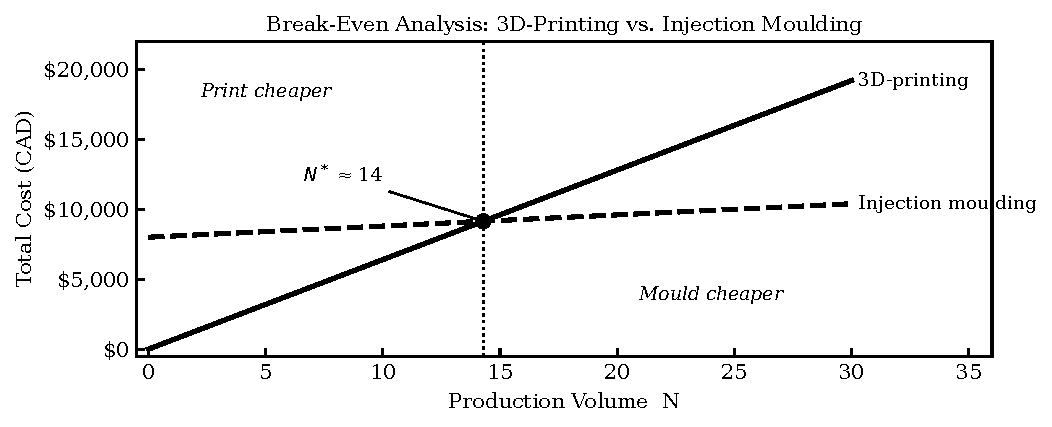
\includegraphics[width=0.82\textwidth]{images/fig_02_breakeven}
  \caption{Total cost for 3D printing and injection moulding as a function of
           production volume.
           The lines cross at $N^{*} = 15$ units.
           Below 15~units the printed process is cheaper; above 15~units the
           moulded process is cheaper.
           The shaded zone around $N^{*}$ represents the indifference region
           where process selection should be driven by lead-time, quality, and
           risk rather than cost alone.}
  \label{fig:ch12-breakeven}
\end{figure}

\subsection{Worked Example B: 3D-Printing vs.\ Injection Moulding}
\label{sec:ch12-worked-b}

The sorting subsystem housing can be produced by either process:

\begin{itemize}
  \item \textbf{Process~1 --- FDM 3D printing:} no tooling required,
        $C_{f1} = \$0$~CAD; per-unit material plus machine time,
        $c_{v1} = \$640$~CAD.
  \item \textbf{Process~2 --- injection moulding:} single-cavity aluminium tool,
        $C_{f2} = \$8{,}000$~CAD; cycle time and material per shot,
        $c_{v2} = \$80$~CAD.
\end{itemize}

Apply Equation~\ref{eq:ch12-breakeven}:

\[
  N^{*} = \frac{C_{f2} - C_{f1}}{c_{v1} - c_{v2}}
         = \frac{8{,}000 - 0}{640 - 80}
         = \frac{8{,}000}{560}
         \approx 14.3 \text{ units.}
\]

Because a fractional unit is not physically meaningful, round up:
$N^{*} = 15$~units.

\medskip
\noindent\textbf{Decision rule:}
\begin{itemize}
  \item Below $N = 15$: use FDM printing.
        Total cost at $N = 10$: printing costs $0 + 10 \times 640 = \$6{,}400$;
        moulding costs $8{,}000 + 10 \times 80 = \$8{,}800$.
        Printing saves \$2,400.
  \item Above $N = 15$: use injection moulding.
        Total cost at $N = 50$: printing costs $0 + 50 \times 640 = \$32{,}000$;
        moulding costs $8{,}000 + 50 \times 80 = \$12{,}000$.
        Moulding saves \$20,000.
\end{itemize}

\paragraph{Common Pitfalls.}
$N^{*}$ is not a sharp switch.
In the neighbourhood of 15~units the cost advantage of either process is small
(a few hundred dollars over the run), while process differences in lead time,
surface finish, and dimensional tolerance can be decisive.
Treat $N^{*}$ as the centre of a zone of indifference --- roughly $\pm$20\,\%
around the calculated value --- and let non-cost factors govern the decision
within that zone.

% ─────────────────────────────────────────────────────────────────────────────
\section{DFM, DFA, and the Design-Locks-Cost Principle}
\label{sec:ch12-dfm-dfa}
% ─────────────────────────────────────────────────────────────────────────────

Chapter~7 introduced Design for Manufacturability and Design for Assembly as
Stage~3 disciplines.
This chapter puts an exact dollar value on each.

\textbf{The design-locks-cost principle}\index{design-locks-cost principle}
states that approximately 70--80\,\% of the lifetime manufacturing cost of a
product is determined by decisions made before the first prototype is built.
Once a geometry is fixed, a component is specified, or an assembly sequence is
locked in, the variable cost $c_{\text{var}}$ is largely set.
Subsequent process optimisation can reduce $c_{\text{var}}$ by a few percent;
only a redesign can change it significantly.

\subsection{DFM Impact on Variable Cost}
\label{sec:ch12-dfm-cvar}

Each DFM decision made in Chapter~7 has a direct entry in $c_{\text{var}}$.
Consider the FDM housing for the sorting subsystem.

\begin{itemize}
  \item \textbf{Wall thickness at 1.5~mm} (above the 1.2~mm minimum): two
        complete perimeters plus a partial infill perimeter.
        Reducing wall thickness to the minimum saves approximately 8\,\% of
        material mass and roughly 12~minutes of print time per unit.
        At a machine rate of \$2.50/hr, this is a saving of \$0.50 per unit ---
        small at 10~units (\$5 total), meaningful at 500~units (\$250 total).
  \item \textbf{Support-free cable channels}: eliminating support material saves
        post-processing labour.
        At \$20/hr labour rate and 8~minutes per unit, the saving is \$2.67 per
        unit, or \$1,335 over 500~units.
\end{itemize}

DFM decisions compound: a design with three or four such improvements can
reduce $c_{\text{var}}$ by 10--15\,\%, shifting the entire unit-cost curve
downward.

\subsection{DFA Impact on Assembly Cost}
\label{sec:ch12-dfa-assembly}

The \textbf{DFA assembly efficiency}\index{DFA assembly efficiency} $\eta_A$
introduced in Chapter~7 quantifies the ratio of theoretically necessary
assembly operations to actual operations.
A low $\eta_A$ means redundant parts, redundant fasteners, or awkward handling
--- all of which inflate the assembly-labour component of $c_{\text{var}}$.

For the sorting subsystem, the housing originally used four M3 screws to secure
the PCB.
Replacing these with two snap-fit latches (a DFA decision from Chapter~7)
reduces the fastener count from four to zero, saves approximately 3~minutes of
assembly time per unit, and removes four BOM line items.
At 500~units this represents 25~hours of assembly labour --- roughly \$500 in
direct savings, plus the reduction in torque-tool calibration cost.

\paragraph{In Practice.}
DFM and DFA improvements are most valuable when they are identified at
Stage~3, before the design is frozen.
A snap-fit geometry that replaces screws is trivial to implement in CAD before
the mould tool is cut.
It is expensive to retrofit after the tool exists: a mould modification
(``steel-safe'' change) costs \$500--\$2{,}000 and adds 2--4~weeks to the
schedule.
This is the practical meaning of the design-locks-cost principle.

% ─────────────────────────────────────────────────────────────────────────────
\section{Failure Economics}
\label{sec:ch12-failure}
% ─────────────────────────────────────────────────────────────────────────────

A unit-cost analysis that excludes failure rates is optimistic.
\textbf{Yield}\index{yield} is the fraction of produced units that pass
acceptance testing and ship to customers.
A yield of 95\,\% means 5 out of every 100 units are scrapped or reworked,
adding their cost to the run without adding to revenue.

The \textbf{effective variable cost}\index{effective variable cost} under a
yield $Y$ is

\begin{equation}
  c_{\text{eff}} = \frac{c_{\text{var}}}{Y}.
  \label{eq:ch12-effective-cvar}
\end{equation}

At $Y = 0.95$ and $c_{\text{var}} = \$480$:
\[
  c_{\text{eff}} = \frac{480}{0.95} \approx \$505\text{ CAD per shipped unit.}
\]

The \$25 difference appears small; at $N = 500$ shipped units it represents an
additional \$12,500 in unrecovered production cost.

\subsection{Cost of a Design Defect Found Late}
\label{sec:ch12-late-defect}

Figure~\ref{fig:ch12-cost-committed} illustrates the \textbf{cost-committed
curve}\index{cost-committed curve}: the cumulative fraction of lifetime cost
that is locked in at each project phase, plotted against the cost actually
incurred.

\begin{figure}[htbp]
  \centering
  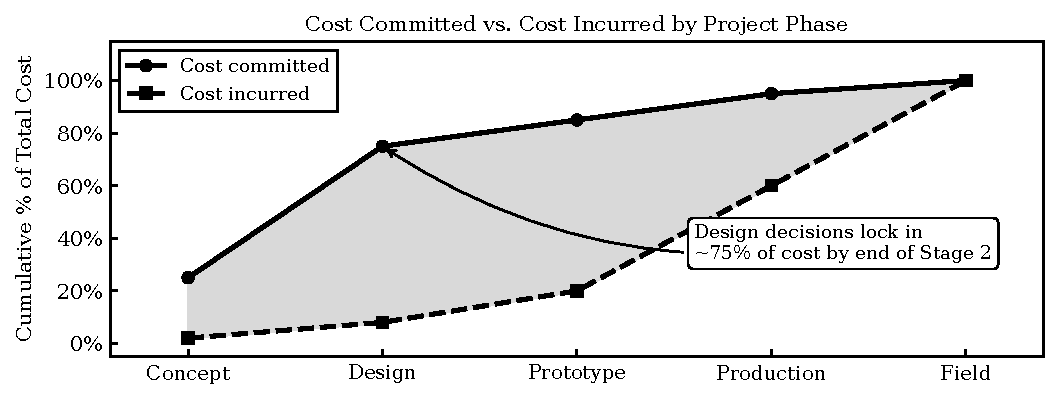
\includegraphics[width=0.82\textwidth]{images/fig_03_cost_committed}
  \caption{Cost committed vs.\ cost incurred over the five Stage-Gate phases.
           By the end of Stage~3 (Development), approximately 75\,\% of
           lifetime manufacturing cost is locked in, yet only 15--20\,\% of
           total project spend has occurred.
           The gap between the two curves is the economic justification for
           intensive front-end design work.}
  \label{fig:ch12-cost-committed}
\end{figure}

A defect found in Stage~3 (a DFA violation, an over-toleranced component, a
housing that requires support material) costs a CAD change and a reprint.
The same defect found in Stage~4, after the mould tool is cut, costs a tool
modification, a delay, and likely a BOM change.
The \textbf{rule of ten}\index{rule of ten} states that the cost of fixing a
defect multiplies by approximately ten at each stage boundary.

% ─────────────────────────────────────────────────────────────────────────────
\section*{Try It Yourself}
\label{sec:ch12-try}
% ─────────────────────────────────────────────────────────────────────────────

A student team is developing a wearable environmental sensor.
The BOM and process estimates give the following parameters:

\begin{itemize}
  \item $C_{\text{fixed}} = \$6{,}000$~CAD (PCB test fixture \$1,800; custom
        enclosure tool \$3,600; NRE \$600).
  \item $c_{\text{var}} = \$35$~CAD per unit (components \$22, assembly
        labour \$13).
  \item Selling price $p = \$199$~CAD.
\end{itemize}

\begin{enumerate}
  \item[(a)] Using Equation~\ref{eq:ch12-unit-cost}, compute $C_{\text{unit}}$
        at $N = 1$, $N = 25$, $N = 100$, and $N = 500$.
        Show every arithmetic step.
  \item[(b)] At what production volume does the fixed-cost contribution per
        unit fall below \$20?
        (Set up the inequality $C_{\text{fixed}}/N < 20$ and solve for $N$.)
  \item[(c)] The team is comparing hand-assembly (soldering iron, jig) against
        contract-manufacturer reflow:
        \begin{itemize}
          \item Hand-assembly: $C_{f1} = \$200$ (jig), $c_{v1} = \$58$~CAD.
          \item CM reflow: $C_{f2} = \$1{,}800$ (setup and stencil),
                $c_{v2} = \$22$~CAD.
        \end{itemize}
        Use Equation~\ref{eq:ch12-breakeven} to find $N^{*}$.
        Round to the nearest whole unit.
        State the decision rule.
  \item[(d)] Yield testing shows 92\,\% of assembled units pass first-pass
        inspection ($Y = 0.92$).
        Compute the effective variable cost $c_{\text{eff}}$ using
        Equation~\ref{eq:ch12-effective-cvar}.
        How does this change the gross margin at $N = 100$?
\end{enumerate}

% ─────────────────────────────────────────────────────────────────────────────
\section*{Review Questions}
\label{sec:ch12-review}
% ─────────────────────────────────────────────────────────────────────────────

\begin{enumerate}
  \item \textbf{(Conceptual)} Explain in one paragraph why a prototype
        unit cost cannot be used directly as the production unit cost.
        Identify at least two cost categories that change between the prototype
        build and a production run of 100~units.

  \item \textbf{(Conceptual)} The design-locks-cost principle states that
        75\,\% of manufacturing cost is committed by the end of Stage~3.
        What practical implication does this have for when DFM and DFA
        reviews should be conducted?
        Why is it economically preferable to discover an assembly violation
        at Stage~3 rather than Stage~4?

  \item \textbf{(Applied --- calculation)} A product has
        $C_{\text{fixed}} = \$12{,}000$~CAD and $c_{\text{var}} = \$75$~CAD.
        Compute $C_{\text{unit}}$ at $N = 20$, $N = 80$, and $N = 400$.
        At what volume does the fixed-cost contribution per unit drop below
        \$50?

  \item \textbf{(Applied --- calculation)} Two enclosure processes are
        available:
        \begin{itemize}
          \item Laser-cut acrylic: $C_{f1} = \$0$, $c_{v1} = \$95$~CAD.
          \item Vacuum-formed HDPE: $C_{f2} = \$3{,}500$~CAD,
                $c_{v2} = \$18$~CAD.
        \end{itemize}
        Use Equation~\ref{eq:ch12-breakeven} to calculate $N^{*}$.
        Show full algebra.
        For a planned run of 60~units, which process minimises total cost,
        and by how much?

  \item \textbf{(Multi-step)} A hardware team projects
        $C_{\text{fixed}} = \$5{,}000$~CAD, $c_{\text{var}} = \$120$~CAD,
        selling price $p = \$350$~CAD, and yield $Y = 0.88$.
        \begin{enumerate}
          \item[(a)] Compute the effective variable cost $c_{\text{eff}}$.
          \item[(b)] Compute $C_{\text{unit}}$ at $N = 50$ using
                $c_{\text{eff}}$ rather than $c_{\text{var}}$.
          \item[(c)] Compute the gross margin $((p - C_{\text{unit}})/p)$
                at $N = 50$.
          \item[(d)] How many units must be produced for the gross margin
                to reach 40\,\%?
                \\\noindent\textit{Hint:} Set $(p - C_{\text{unit}})/p = 0.40$ and solve for $N$, using $c_{\text{eff}}$ in the expression for $C_{\text{unit}}$.
        \end{enumerate}
\end{enumerate}

% ─────────────────────────────────────────────────────────────────────────────
\section*{Portfolio Entry}
\addcontentsline{toc}{section}{Portfolio Entry}
\label{sec:ch12-artifact}
% ─────────────────────────────────────────────────────────────────────────────

The deliverable for this chapter is a \textbf{Preliminary Cost Analysis}\index{preliminary cost analysis} document that will feed directly into the Chapter~17 financial model.
The document must contain the following elements:

\begin{enumerate}
  \item[(a)] \textbf{Parameter table.} State $C_{\text{fixed}}$, $c_{\text{var}}$,
        selling price $p$, and yield $Y$ with sources for each value.

  \item[(b)] \textbf{Unit-cost table.} $C_{\text{unit}}$ at $N = 50$, $N = 100$,
        and $N = 500$, computed from Equation~\ref{eq:ch12-unit-cost}.
        For the sorting subsystem:

        \begin{center}
        \begin{tabular}{rcc}
          \hline
          $N$ & $C_{\text{unit}}$ & Gross margin \\
          \hline
           50 & \$640 CAD & 46.7\,\% \\
          100 & \$560 CAD & 53.3\,\% \\
          500 & \$496 CAD & 58.7\,\% \\
          \hline
        \end{tabular}
        \end{center}

  \item[(c)] \textbf{Process break-even.} Identify the competing processes,
        state $C_{f1}$, $C_{f2}$, $c_{v1}$, $c_{v2}$, compute $N^{*}$ using
        Equation~\ref{eq:ch12-breakeven}, and state the decision rule.

  \item[(d)] \textbf{DFM/DFA flags.} List at least two design decisions from
        your Stage~3 review (Chapter~7) that affect $c_{\text{var}}$, and
        quantify the per-unit and per-run impact at $N = 100$.

  \item[(e)] \textbf{Gate~3 recommendation.} One sentence: given the unit-cost
        curve and the selling price, does the economics support proceeding to
        Stage~4?
\end{enumerate}

% ─────────────────────────────────────────────────────────────────────────────
\section*{Chapter Summary}
\label{sec:ch12-summary}
% ─────────────────────────────────────────────────────────────────────────────

Low-volume production economics turns on a single equation: fixed costs spread over the run, variable costs paid per unit, yielding a hyperbolic unit-cost curve that falls steeply below 50~units and flattens toward $c_{\text{var}}$ above 100.
Fixed costs ($C_{\text{fixed}}$) are paid once and spread over the run;
variable costs ($c_{\text{var}}$) scale with every unit.
Their combination produces the unit-cost curve (Equation~\ref{eq:ch12-unit-cost}),
a hyperbola that falls steeply at low volume and flattens toward $c_{\text{var}}$
at high volume.
For the sorting subsystem ($C_{\text{fixed}} = \$8{,}000$~CAD,
$c_{\text{var}} = \$480$~CAD), unit cost drops from \$640 at 50~units to
\$496 at 500~units --- a 22\,\% improvement that is already 97\,\% of the
maximum possible gain from volume scaling alone.

Process break-even (Equation~\ref{eq:ch12-breakeven}) showed that injection
moulding becomes cheaper than FDM printing at $N^{*} = 15$~units for the
housing, but that $N^{*}$ should be treated as a zone rather than a sharp
switch.

The design-locks-cost principle connects this chapter directly to Chapter~7:
DFM and DFA decisions made at Stage~3 set $c_{\text{var}}$ for the lifetime of
the product.
The cost-committed curve confirms that front-end design investment is the
highest-return activity available to the team.

You now have a Preliminary Cost Analysis with $C_{\text{unit}}$ at $N = 50$,
$N = 100$, and $N = 500$, a process break-even decision, and a Gate~3
recommendation.
Chapter~13 takes that full design package and shows how to establish a version-controlled design history file --- the Configuration Management Record --- so that every artefact can be recovered, compared, and audited as the design evolves toward the Stage~4 release.
